\documentclass[a4paper]{report}

\usepackage{amsmath} % for the equation* environment

\title{Vaja 16 Vztrajnostni moment}
\author{Jure Kos}
\date{14.10.2021}
\usepackage{graphicx}
\graphicspath{{./images/}}

\begin{document}

\maketitle
\chapter*{Uvod}
Togo telo, ki je vrtljivo okoli nepremične osi, se vrti enakomerno pospešeno, če deluje nanj konstanten navor v smeri osi. Kotni pospešek  \textit{$\alpha$} in navor \textit{M} sta sorazmerna:

\[J\alpha=M\]

Pri tem je \textit{J} vztrajnostni moment telesa okoli dane osi, ki ga določa porazdelitev mase telesa \textit{$\delta m_i$} glede na oddaljenost od osi vrtenja \textit{$r_i$} po formuli
\[J=\sum_{i}r_i^2 \Delta m_i \Rightarrow \int_{V} r^2 dm \Rightarrow \int_{V} \rho (r)r^2 dV \]
kjer je \textit{$ \rho (r)$} gostota na mestu \textit{r}. Tako je vztrajnostni moment valjastega kolesa z radijem \textit{R} glede na lastno os enak

\[J=\frac{1}{2}mR^2\]

Kadar pa se vrti okoli osi, ki je vzporedna lastni, toda premaknjena za \textit{$R_p$}, dobimo iz enačbe vztrajnostni moment kot

\[J=\frac{1}{2}mR^2+mR_p^2\]

Okoli vodoravne osi vrtljivo kolo poganjamo z utežjo preko vrvice, ki je navita na jermenico z radijem \textit{$r_j$} . Utež se giblje s pospeškom

\[a=g-\frac{T}{m_u}\]

kjer sila \textit{T} napenja vrvico in povzroča na kolesu navor \textit{$r_j T$}. Kotni pospešek kolesa dobimo iz zveze

\[J\alpha=r_j m_u (g-a)=m_u (r_j g-r_j^2 \alpha)\]

ali

\[(J+r_j^2 m_u)\alpha=r_j m_u g\]

kjer je \textit{J} skupni vztrajnostni moment kolesa, jermenice in morebitnih dodatkov pritrjenih na kolo. Poglejmo še, kako je z izrekom o kinetični energiji pri tem poskusu! Spočetka kolo in utež mirujeta. Ko se spusti utež za višino \textit{h}, se kolo vrti s kotno hitrostjo $\omega$. Kinetična energija sistema je enaka spremembi potencialne energije uteži

\[m_u gh=J\frac{\omega^2}{2}+\frac{m_u v_u^2}{2}\]

kjer predstavlja zadnji člen kinetično energijo uteži. Odtod dobimo enačbo:

\[\frac{1}{2}[J+m_ur_j^2]\omega^2=m_u gh\]


\section*{Naloga}

1. Preveriti, da je vrtenje, ki ga povzroča konstanten navor, enakomerno pospešeno
in iz pospeška določiti vztrajnostni moment praznega kolesa.\\
2. Iz pospeška določiti vztrajnostni moment priprave, potem ko smo vpeli manjši
kolesi najprej\\
(a) togo in potem\\
(b) gibljivo v krogljična ležaja.\\
Izračunati nova vztrajnostna momenta še iz podatkov za manjši kolesi in obe vrednosti primerjati!\\
3. Preveriti veljavnost izreka o kinetični energiji.

\section*{Potrebščine}

1. Kolo z jermenico,\\
2. dva para manjših koles,\\
3. uteži,\\
4. vrvica,\\
5. detektor časovnih intervalov (optična vrata),\\
6. zapisovalnik rezultatov (računalnik z ustreznim vmesnikom).
\chapter*{Meritve}
Masa malih koles:\\
$m= 515g \pm 1g$\\
\noindent Masa uteži:\\
$m=50g \pm 1g$\\
\noindent Višina mize:\\
$h=100cm \pm 1cm$\\
\noindent Radij velikega kolesa:\\
$R=5cm \pm 0,1cm$\\
\noindent Radij malih koles:\\
$r=14cm \pm 0,1cm$\\
\noindent Oddaljenost malih koles od središča:\\
$h=7,3cm \pm 0,1cm$\\
\noindent Ročica navora sile teže:\\
$r_g = 2cm \pm 0,1cm$\\

\chapter*{Računi}
Iz izmerjenih kotnih pospeškov lahko za vsako verzijo poskusa izračunamo J:

\[J=\frac{r_g m_u (g-r_g\alpha)}{\alpha}=r_g m_u(\frac{g}{\alpha}-r_g)\]

\noindent Dobimo naslednje rezultate:

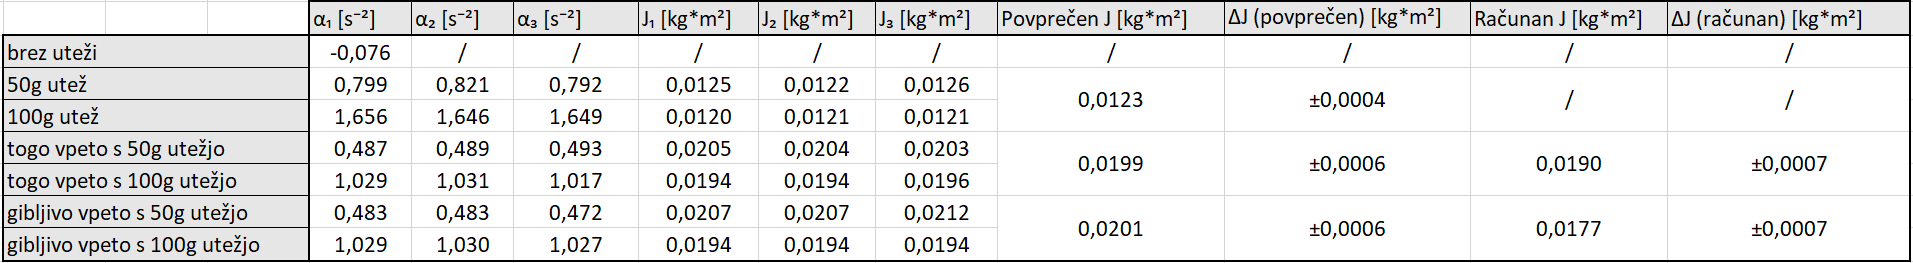
\includegraphics[width = \textwidth]{Tabela}


\chapter*{Grafi}

\noindent Grafi razdalje, hitrosti in pospeška za navor trenja\\
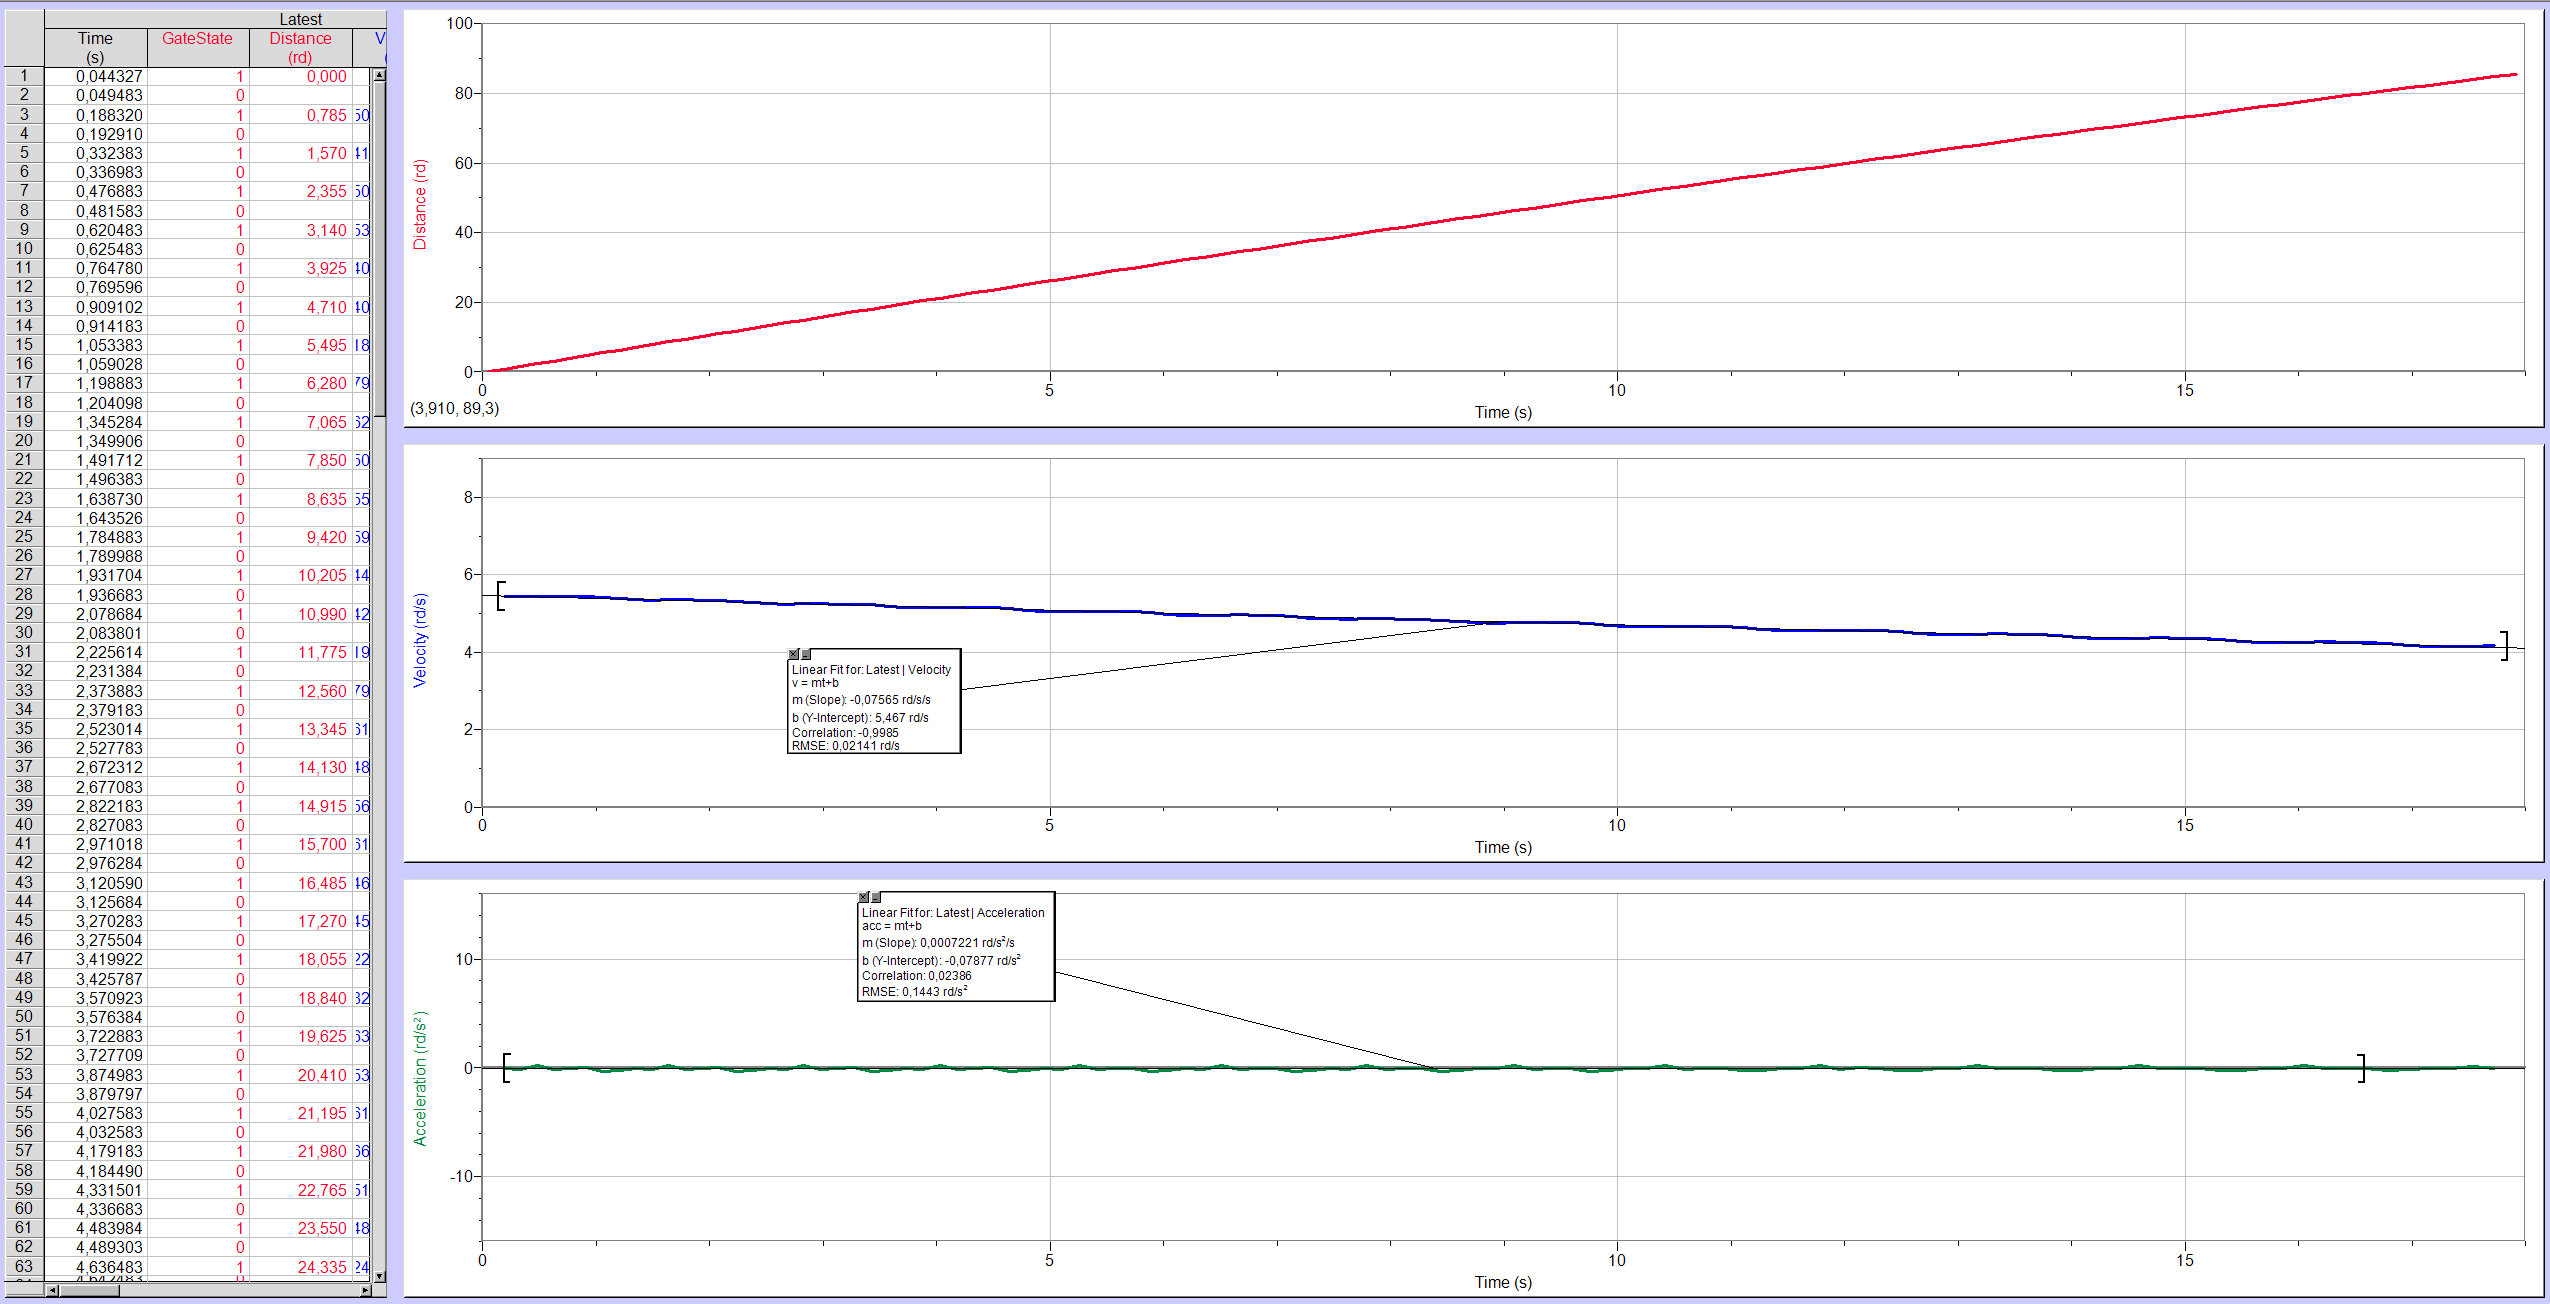
\includegraphics[width = \textwidth]{Trenje}\\

\noindent Grafi razdalje, hitrosti in pospeška za 50g utež\\
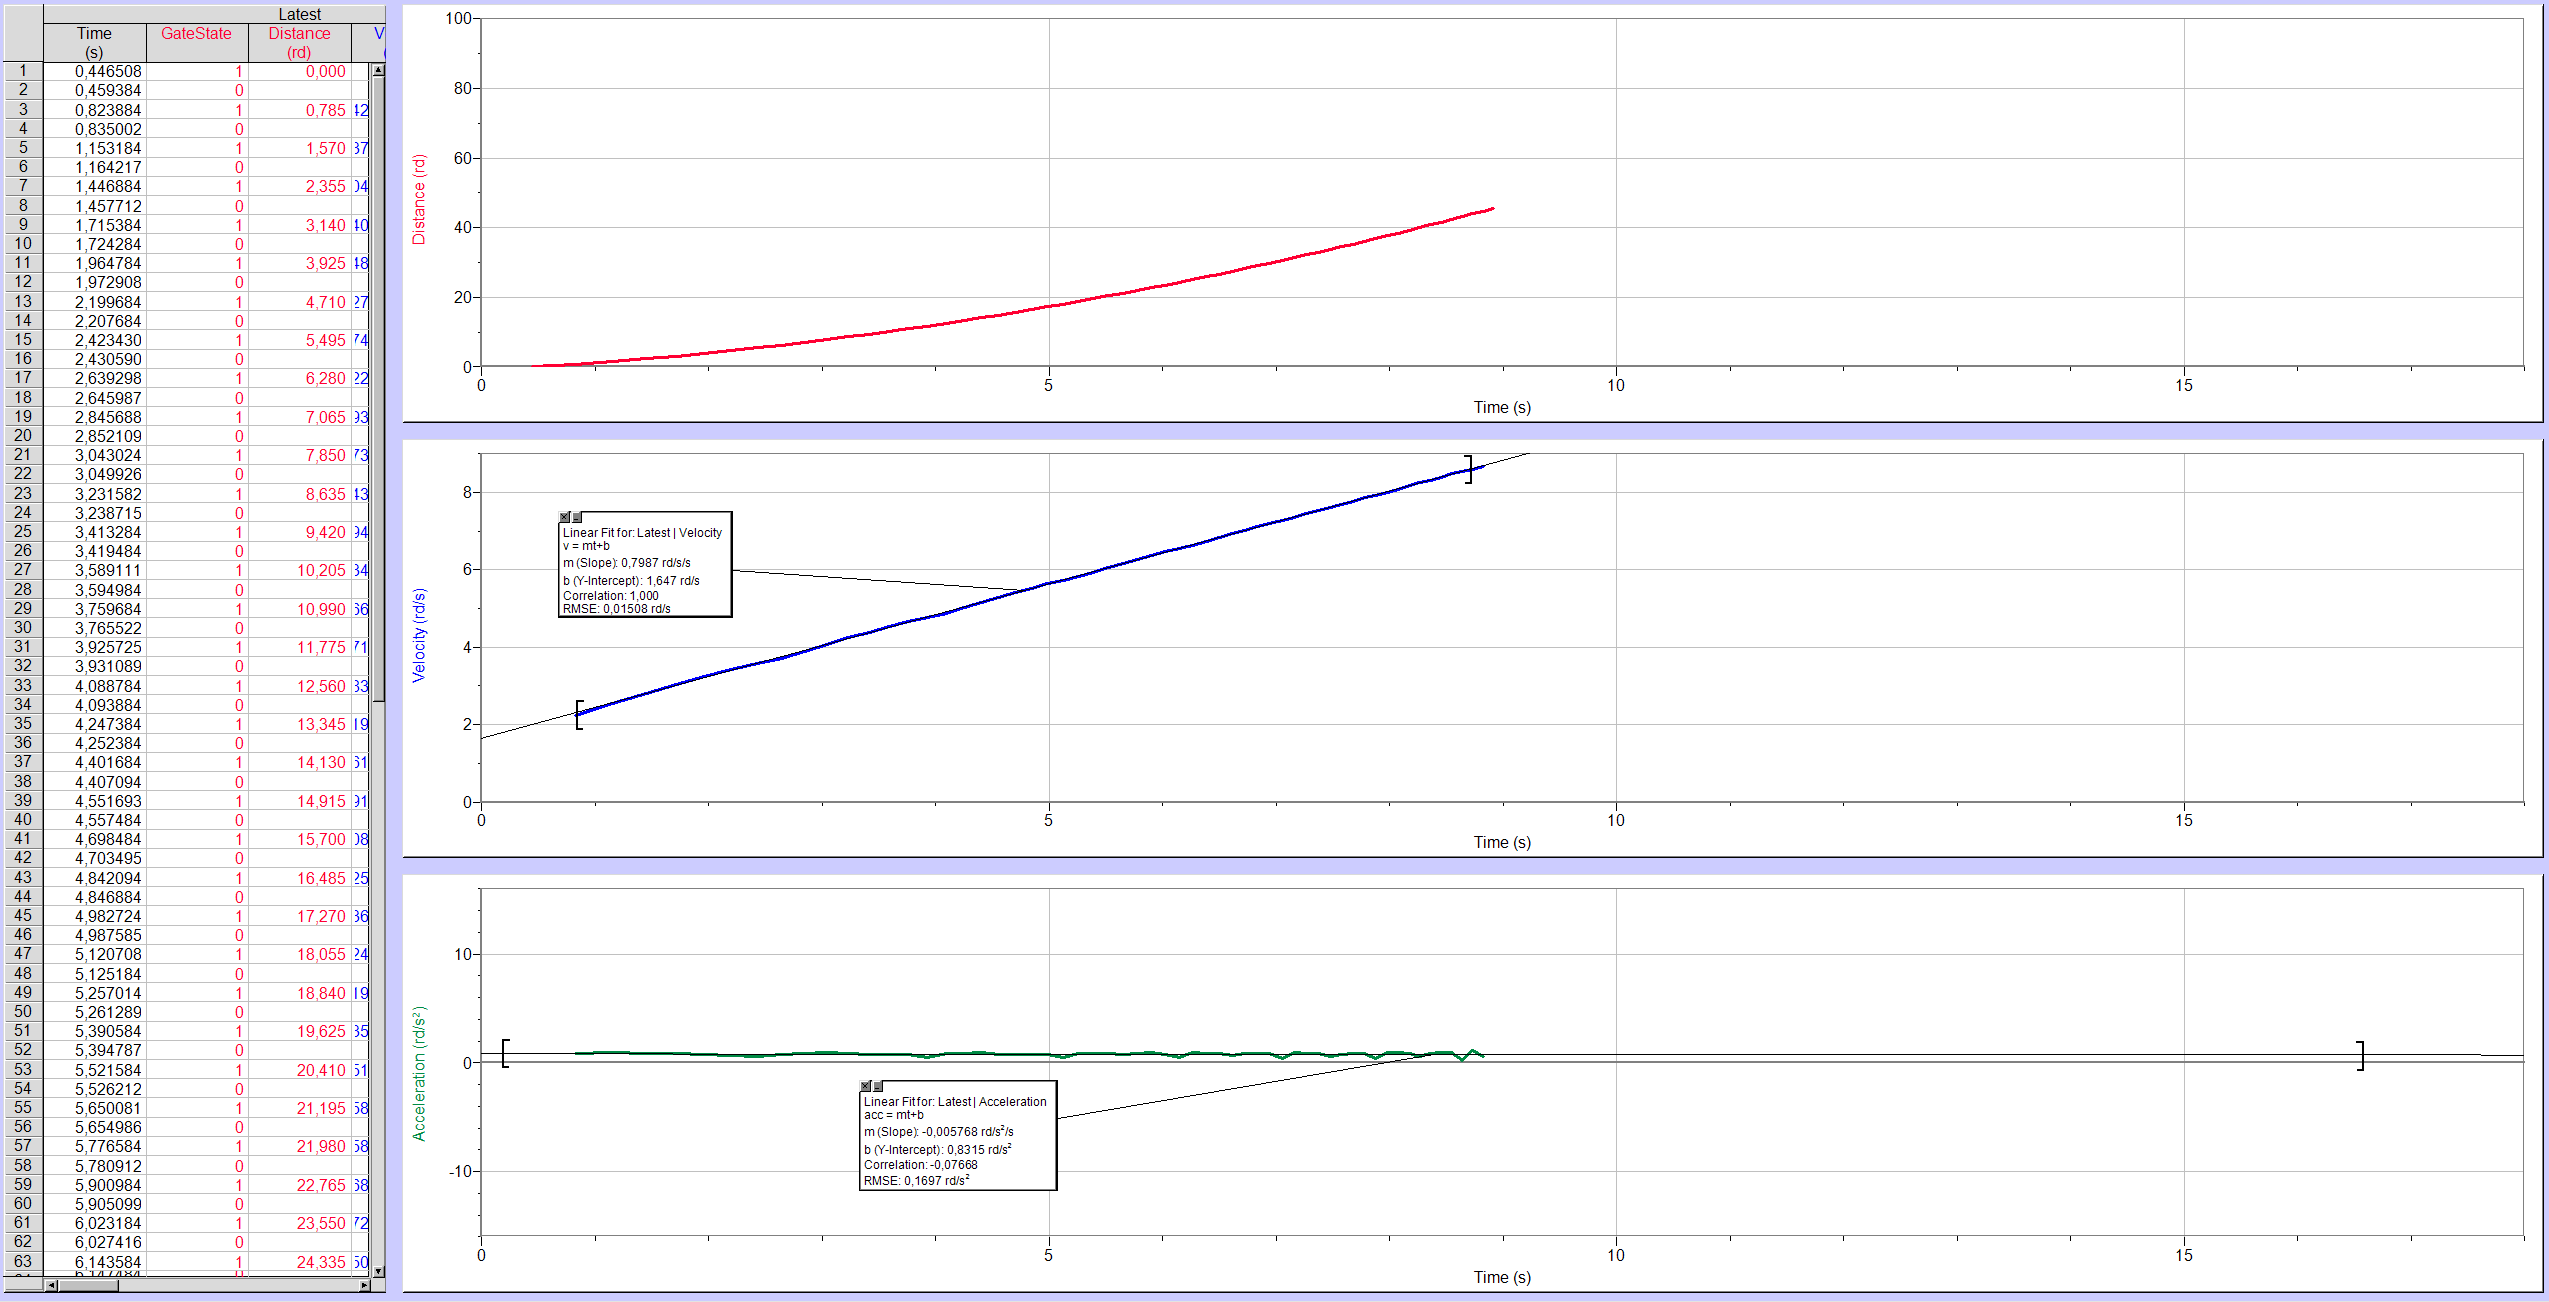
\includegraphics[width = \textwidth]{50g}\\
 
\pagebreak
\noindent Grafi razdalje, hitrosti in pospeška za 100g utež\\
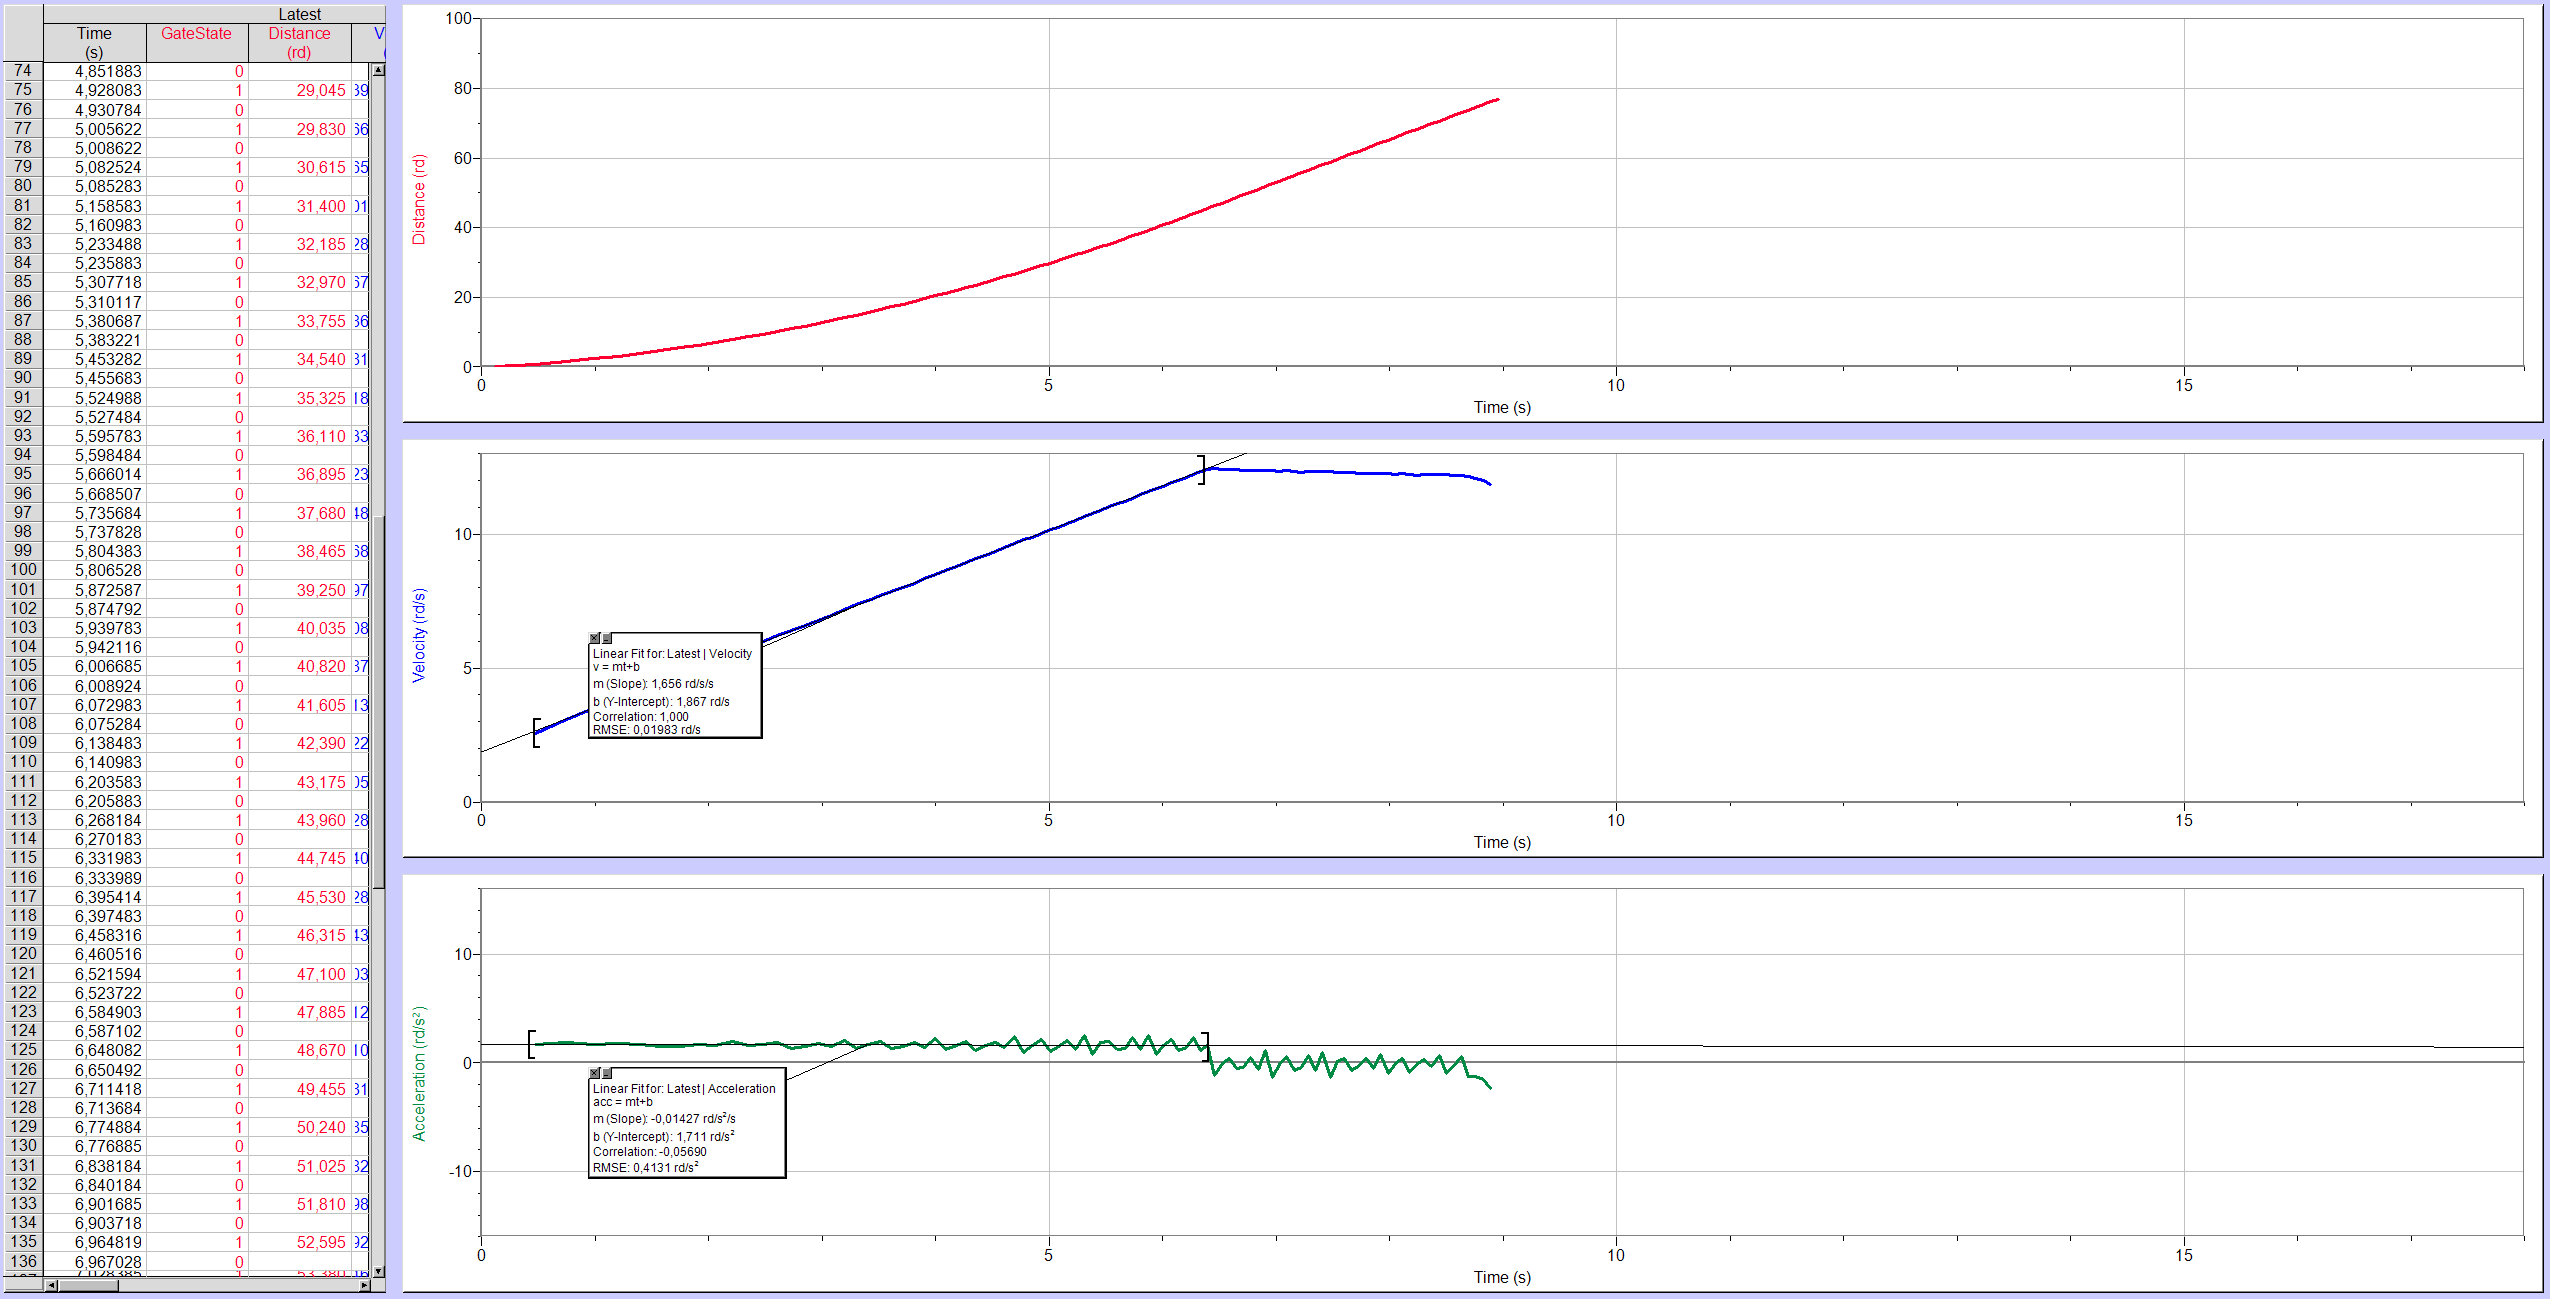
\includegraphics[width = \textwidth]{100g}\\

\noindent Grafi razdalje, hitrosti in pospeška za 50g utež in togo vpete diske\\
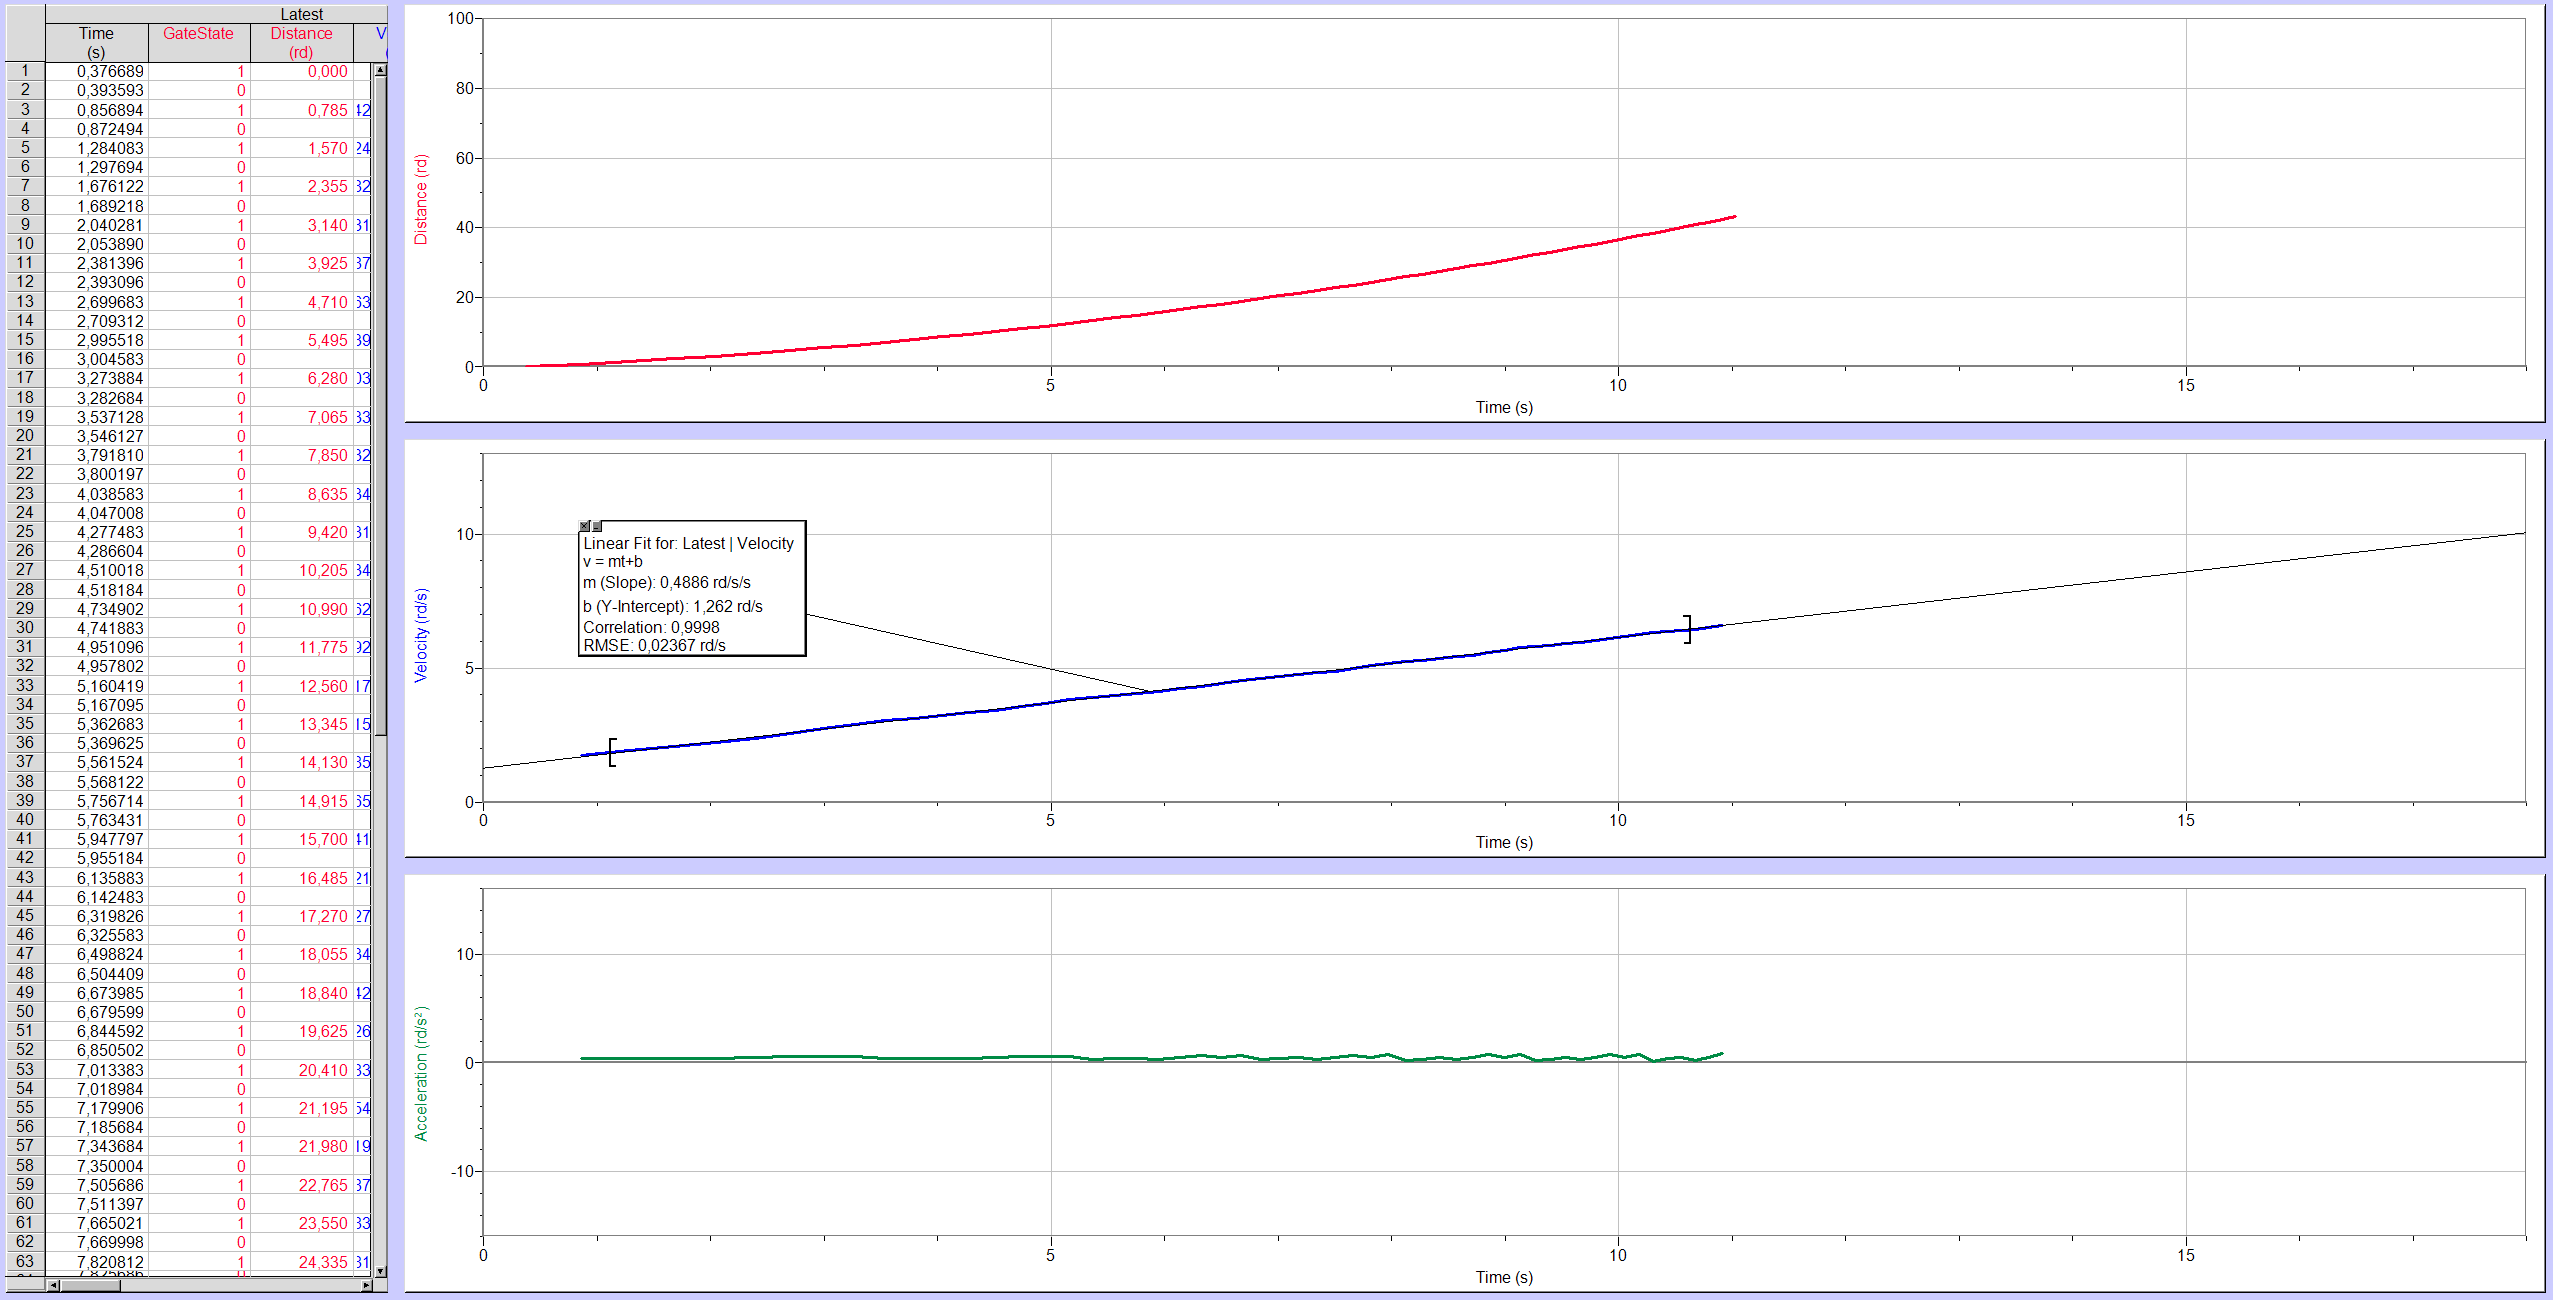
\includegraphics[width = \textwidth]{Togo 50g}\\

\noindent Grafi razdalje, hitrosti in pospeška za 100g utež in togo vpete diske\\
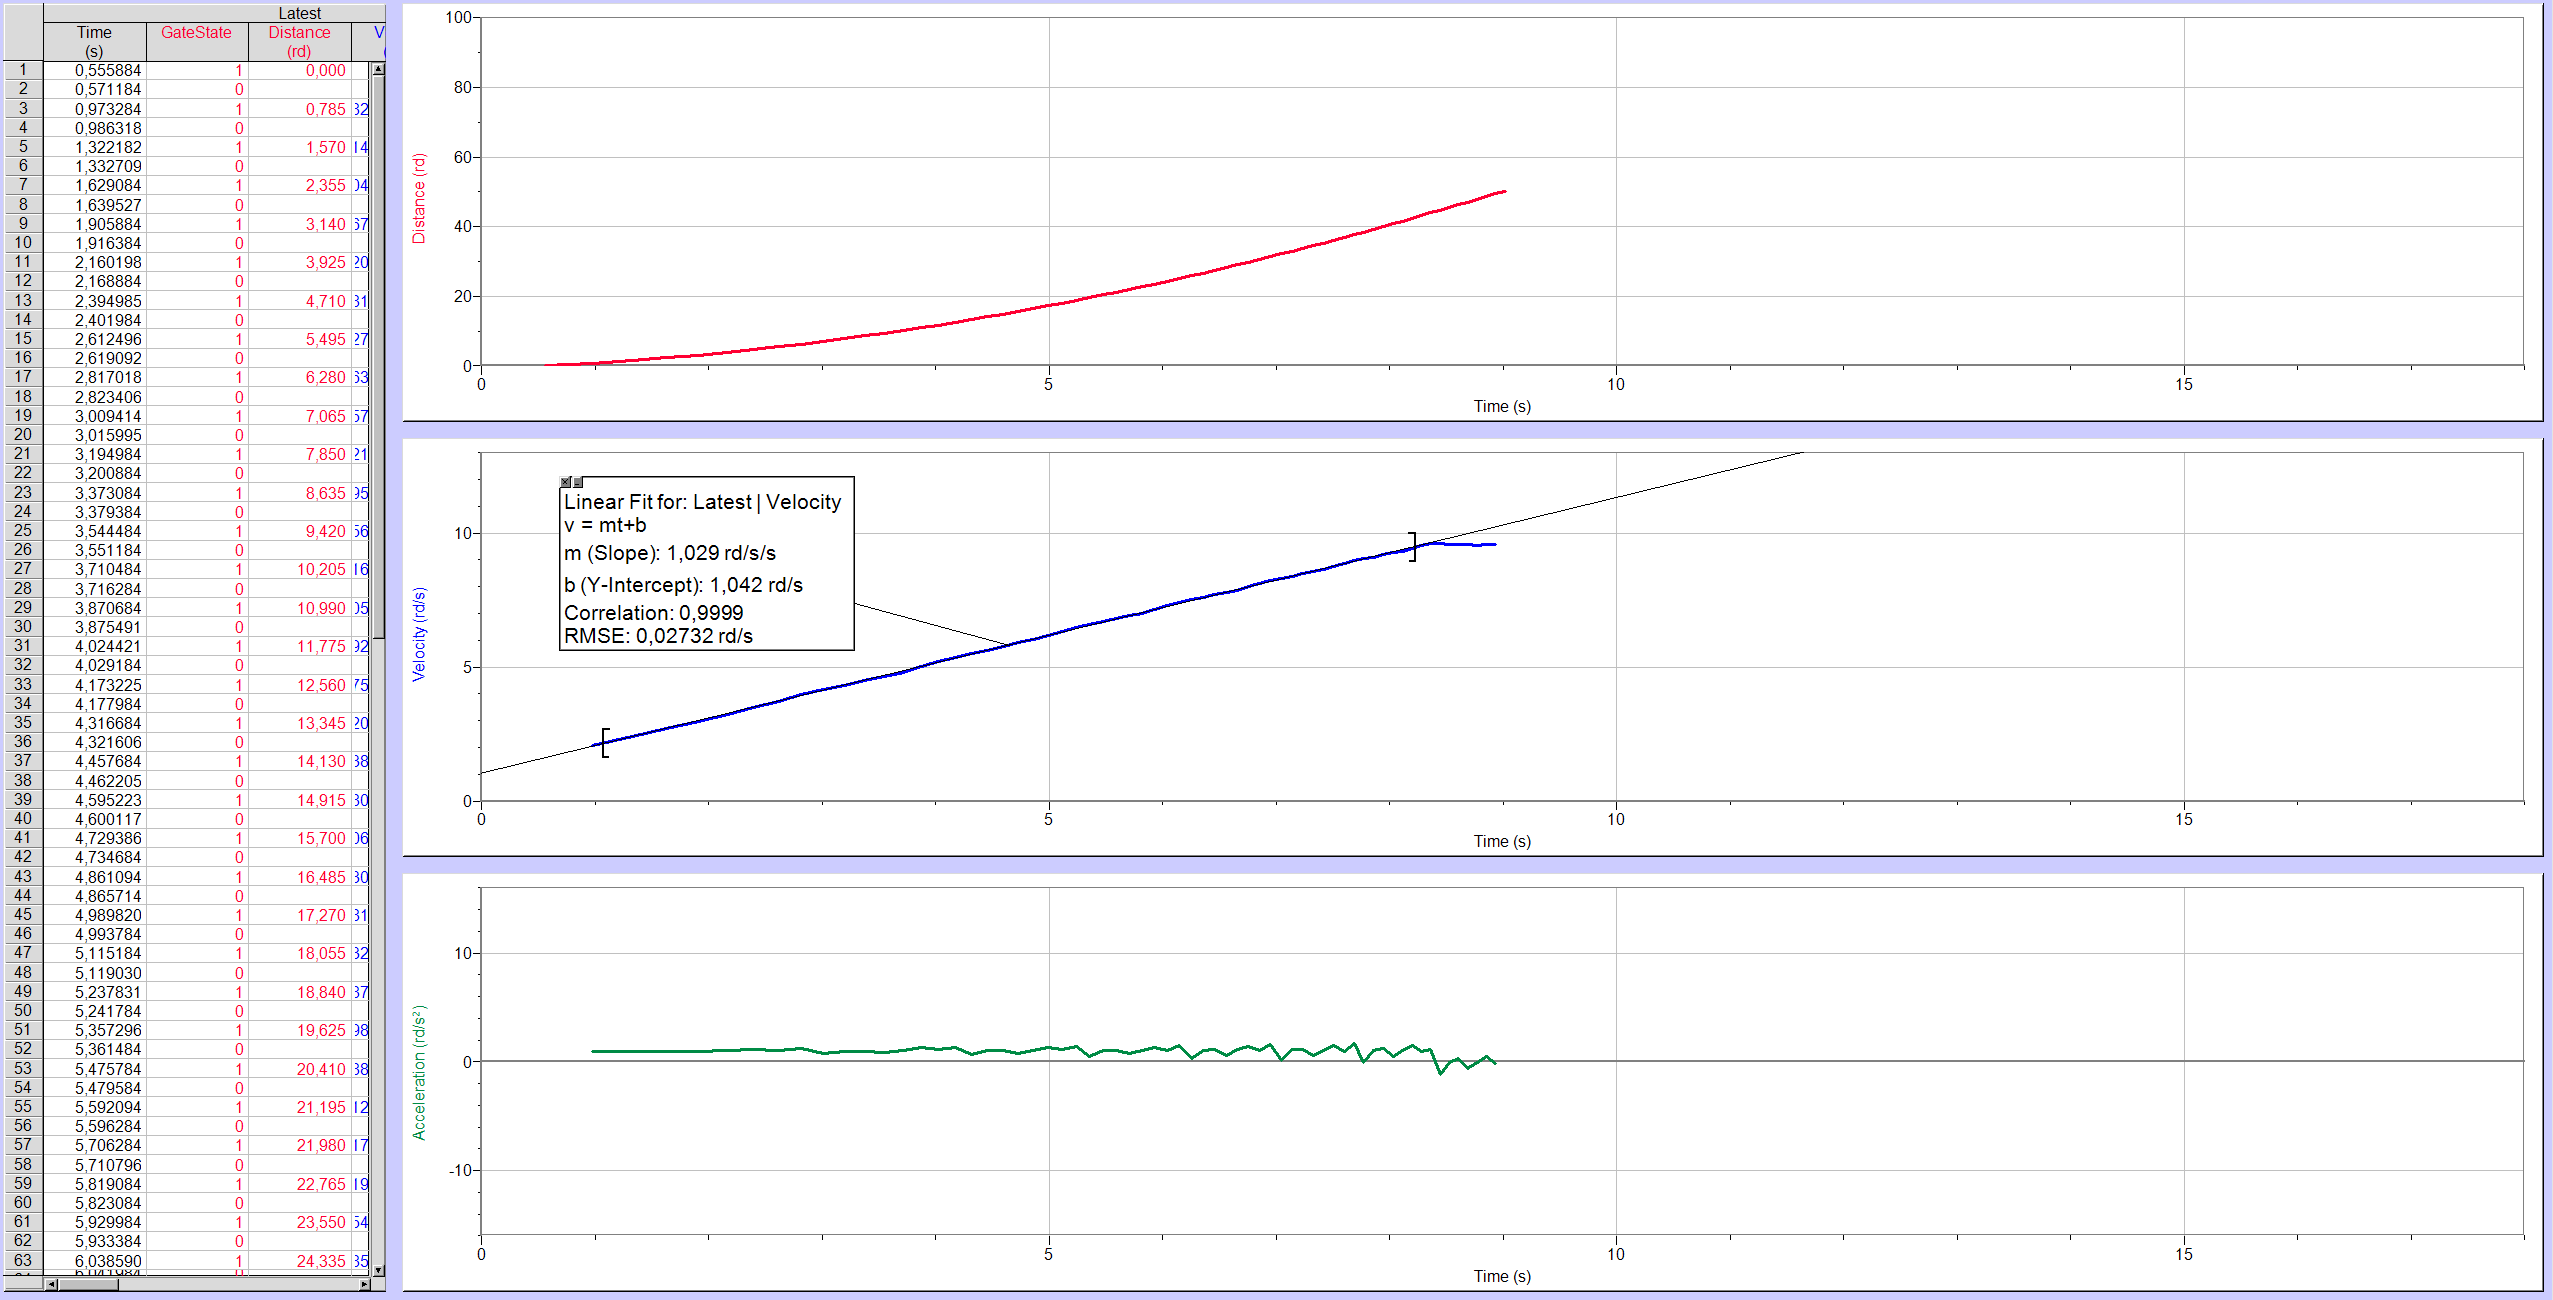
\includegraphics[width = \textwidth]{Togo 100g}\\

\noindent Grafi razdalje, hitrosti in pospeška za 50g utež in gibljivo vpete diske\\
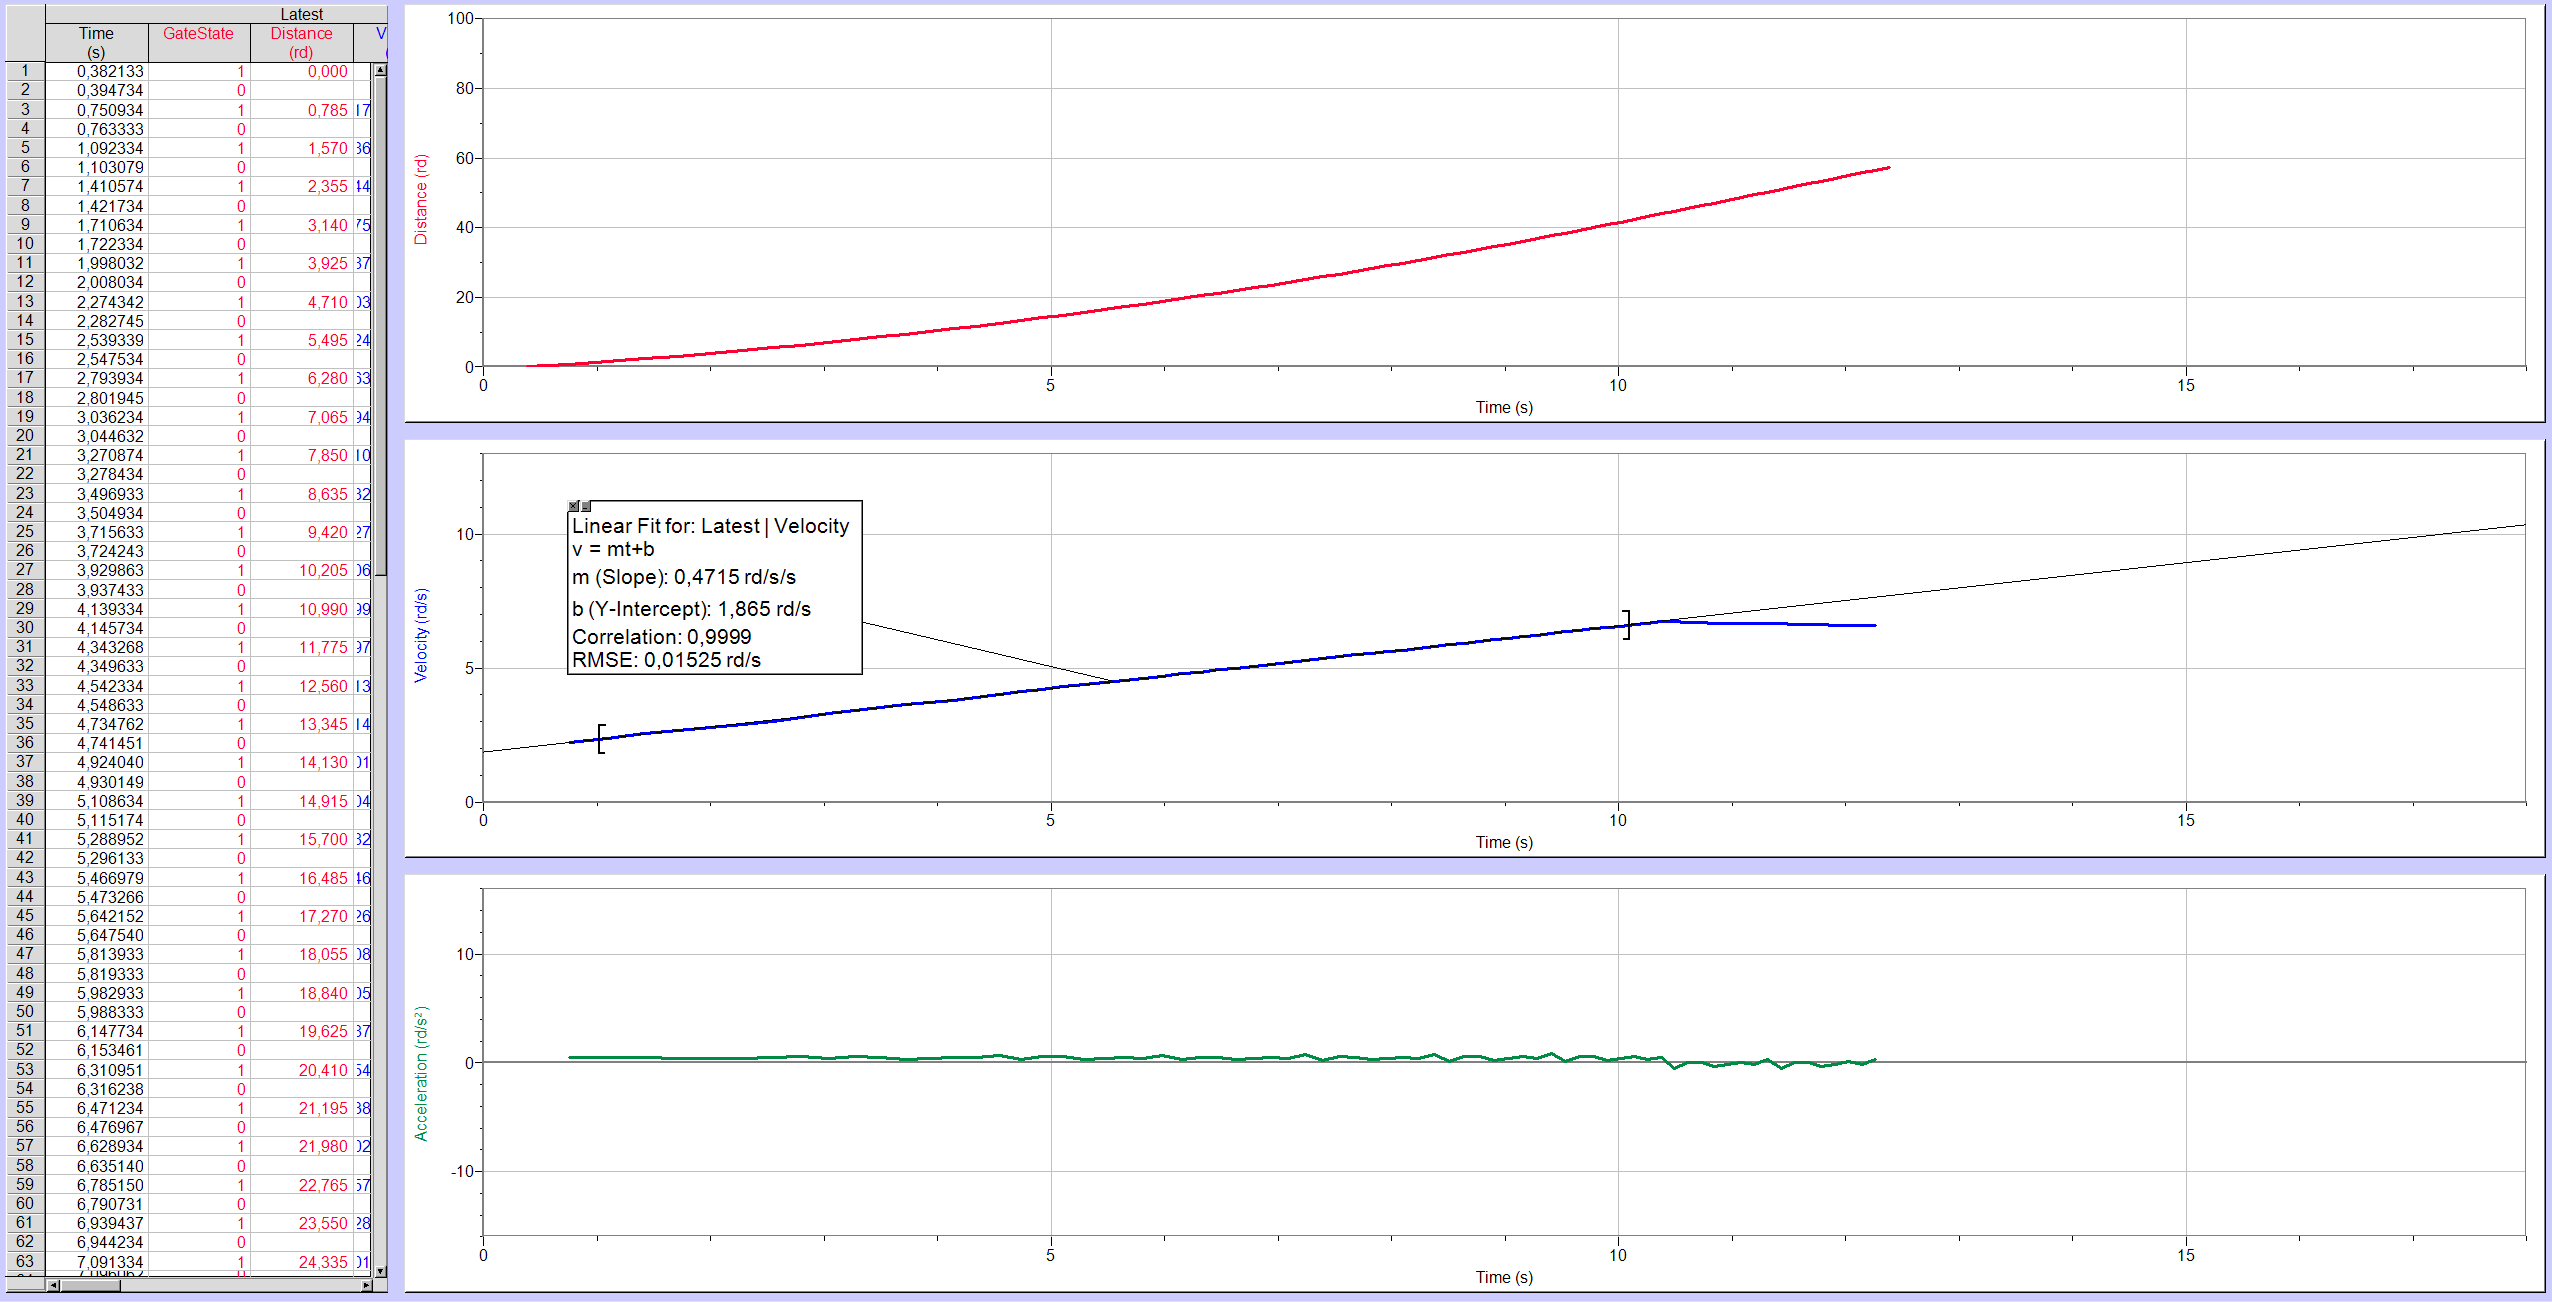
\includegraphics[width = \textwidth]{Gibljivo 50g}\\

\noindent Grafi razdalje, hitrosti in pospeška za 100g utež in gibljivo vpete diske\\
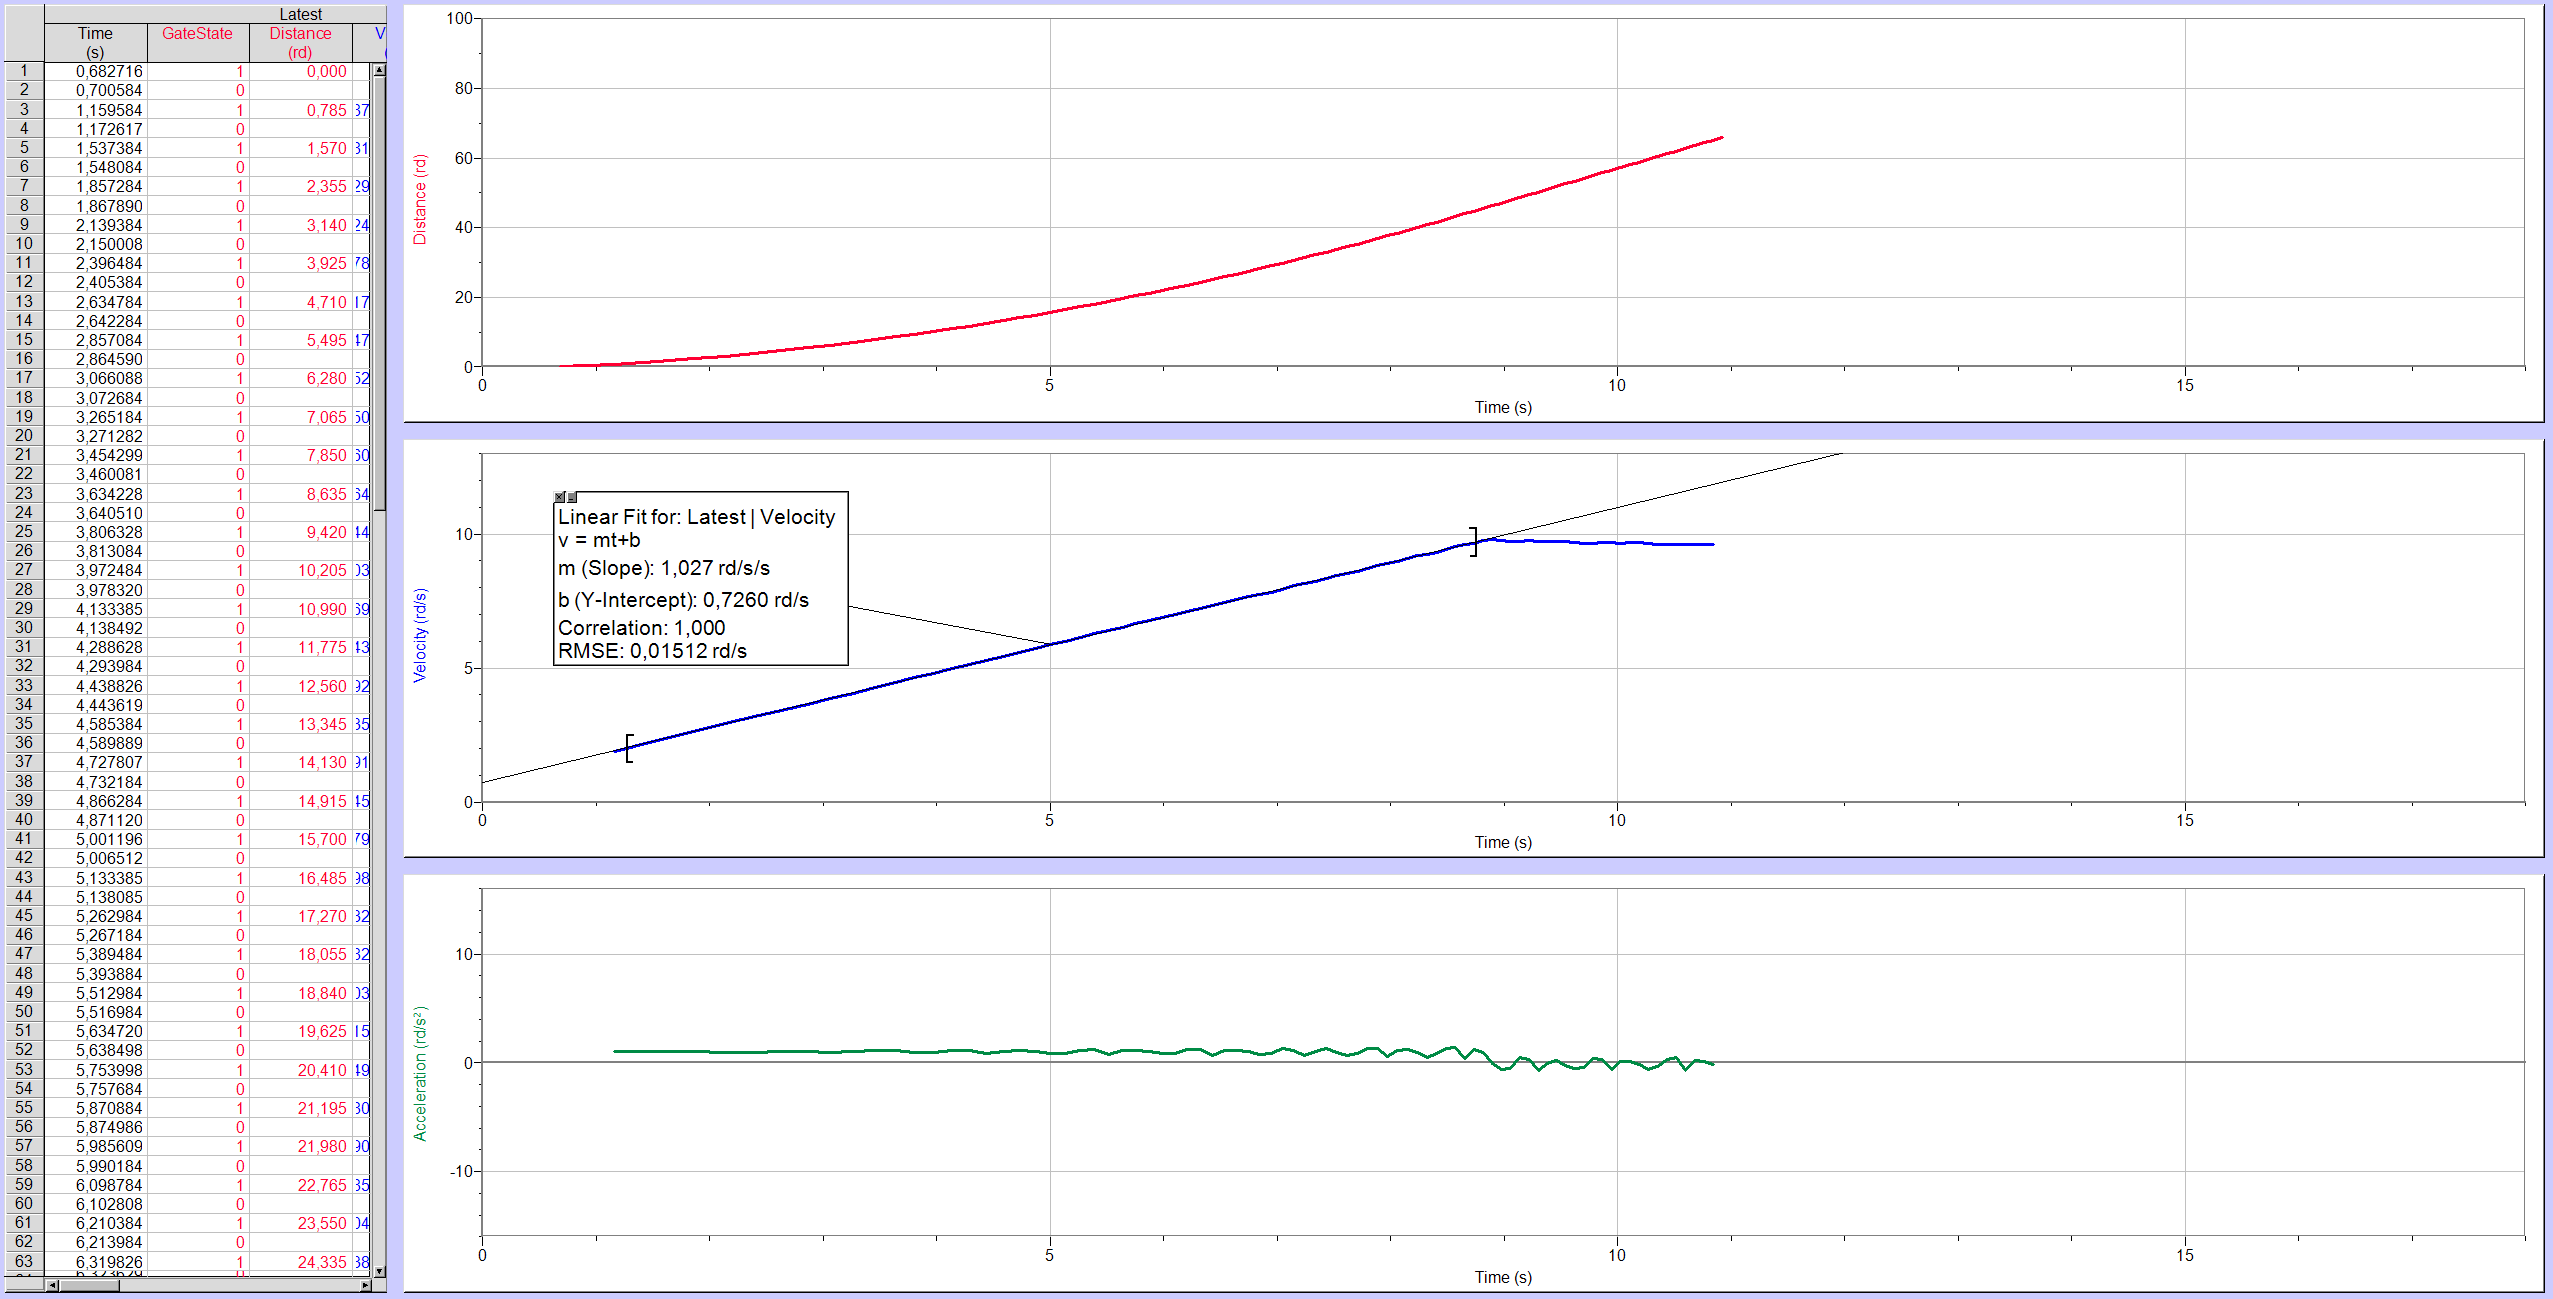
\includegraphics[width = \textwidth]{Gibljivo 100g}

\end{document}